\documentclass[twocolumn,a4j]{jsarticle}
\setlength{\topmargin}{-20.4cm}
\setlength{\oddsidemargin}{-10.4mm}
\setlength{\evensidemargin}{-10.4mm}
\setlength{\textwidth}{18cm}
\setlength{\textheight}{26cm}

\usepackage[top=15truemm,bottom=20truemm,left=20truemm,right=20truemm]{geometry}
\usepackage[latin1]{inputenc}
\usepackage{amsmath}
\usepackage{amsfonts}
\usepackage{amssymb}
\usepackage[dvipdfmx]{graphicx}
\usepackage[hang,small,bf]{caption}
\usepackage[subrefformat=parens]{subcaption}
\usepackage[dvipdfmx]{color}
\usepackage{listings}
\usepackage{listings,jvlisting}
\usepackage{geometry}
\usepackage{framed}
\usepackage{color}
\usepackage[dvipdfmx]{hyperref}
\usepackage{ascmac}
\usepackage{enumerate}
\usepackage{tabularx}
\usepackage{cancel}
\usepackage{scalefnt}
\usepackage{overcite}
\usepackage{otf}
\usepackage{multicol}
\usepackage[geometry]{ifsym}

\renewcommand{\figurename}{Fig.}
\renewcommand{\tablename}{Table }

\hypersetup{%
    hidelinks %リンクの色消し
}

\lstset{
basicstyle={\ttfamily},
identifierstyle={\small},
commentstyle={\smallitshape},
keywordstyle={\small\bfseries},
ndkeywordstyle={\small},
stringstyle={\small\ttfamily},
frame={tb},
breaklines=true,
columns=[l]{fullflexible},
xrightmargin=0zw,
xleftmargin=3zw,
numberstyle={\scriptsize},
stepnumber=1,
numbersep=1zw,
lineskip=-0.5ex
}

% キャプション後ろのダブルコロンを消す
\makeatletter
\long\def\@makecaption#1#2{%
  \vskip\abovecaptionskip
  \iftdir\sbox\@tempboxa{#1\hskip1zw#2}%
    \else\sbox\@tempboxa{#1 #2}%
  \fi
  \ifdim \wd\@tempboxa >\hsize
    \iftdir #1\hskip1zw#2\relax\par
      \else #1 #2\relax\par\fi
  \else
    \global \@minipagefalse
    \hbox to\hsize{\hfil\box\@tempboxa\hfil}%
  \fi
  \vskip\belowcaptionskip}
\makeatother


\makeatletter
\def\@maketitle
{
\begin{center}
{\LARGE \@title \par}
\end{center}
\begin{flushright}
{\large \@date}\\
{\large 京都工芸繊維大学 大学院 機械設計学専攻 計測システム工学研究室}\\
{\large M2 \@author}
\end{flushright}
\par\vskip 1.5em
}
\makeatother

\author{来代 勝胤 / KITADAI Masatsugu}
\title{令和5年度 7月度 共同研究報告書}
\date{2023/07/25}

\begin{document}
\columnseprule=0.1mm
\maketitle

\section*{報告内容}
\begin{enumerate}[1.]
  \item 二次流れの計測実験
  \item 可視化情報シンポジウム 資料作成
  \item 8月の予定
\end{enumerate}

\section*{進捗報告}
今月は,可視化情報シンポジウムの発表に向けた実験と資料作成を行った.
また,二次流れの解析において,
正しい時刻差の粒子像の組み合わせを選択するための
アルゴリズムの検討の検討を行っている.

\section{二次流れの計測実験}

今週は可視化情報シンポジウムの資料作成に向けた
二次流れの撮影実験を行った.
三角翼モデルについて渦構造の乱れが少ないと考えられる
後端直後の流れについて,右翼部および中央部,
車両モデル車軸部の測定結果の解析を行った.
以下の Table.1 に実験条件を示す.
また,撮影できる粒子像の増加を期待し,
カメラのゲイン(撮影時の明るさ)を変更して
+0, +5, +10 の3パターンについて撮影を行った.

\begin{table}[hbtp]
  \centering
  \caption{Experimental conditions}
  \begin{tabular}{ c r l }
    \hline
    Mainstream velocity              & 250  & mm/s \\ \hline
    Frame rate                       & 800  & fps  \\ \hline
    Shutter speed                    & 1000 & 1/s  \\ \hline
    Thickness of LLS 1               & 1.0  & mm   \\ \hline
    Thickness of LLS 2               & 3.0  & mm   \\ \hline
    Distance between LLS 1 and LLS 2 & 2.5  & mm   \\ \hline
    Shooting time                    & 5    & s    \\ \hline
  \end{tabular}
\end{table}

\newpage
\subsection{三角翼後流(1) 右翼部}
これまで,後端部から 50 mm の位置について
計測を行ってきたが,外乱による渦構造の変化や崩壊の可能性を考慮し
後端部直後(後端部から 0 mm の位置)の撮影を行った.
それらの解析結果をFig.1に示す.

\begin{figure}[htbp]
  \footnotesize
  \begin{center}
    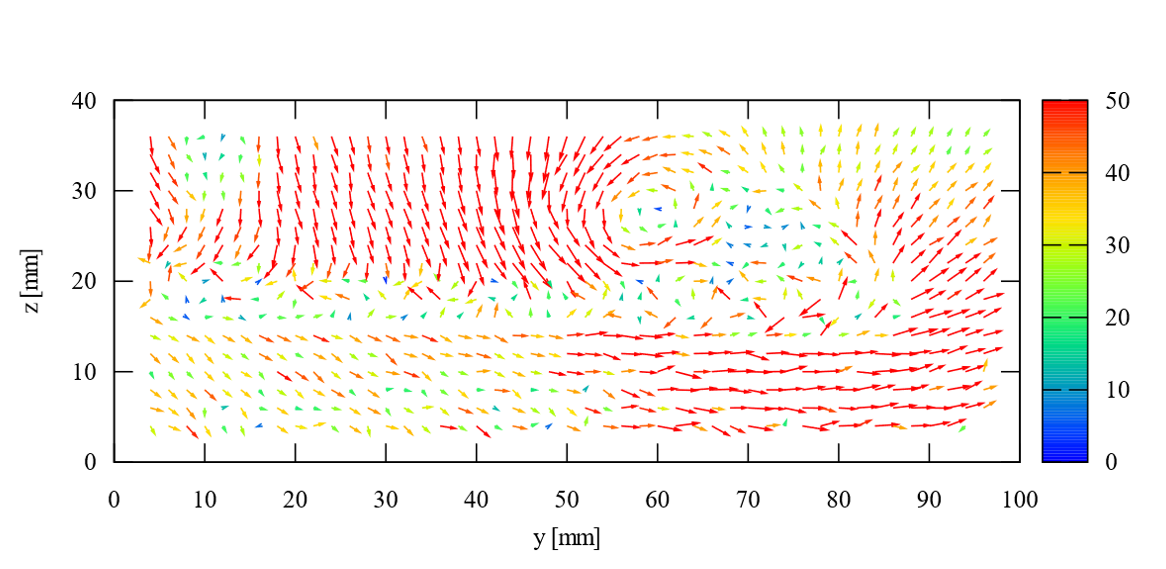
\includegraphics[width=82mm]{../images/right_+0.png}
    \subcaption{Gain $+0$}
    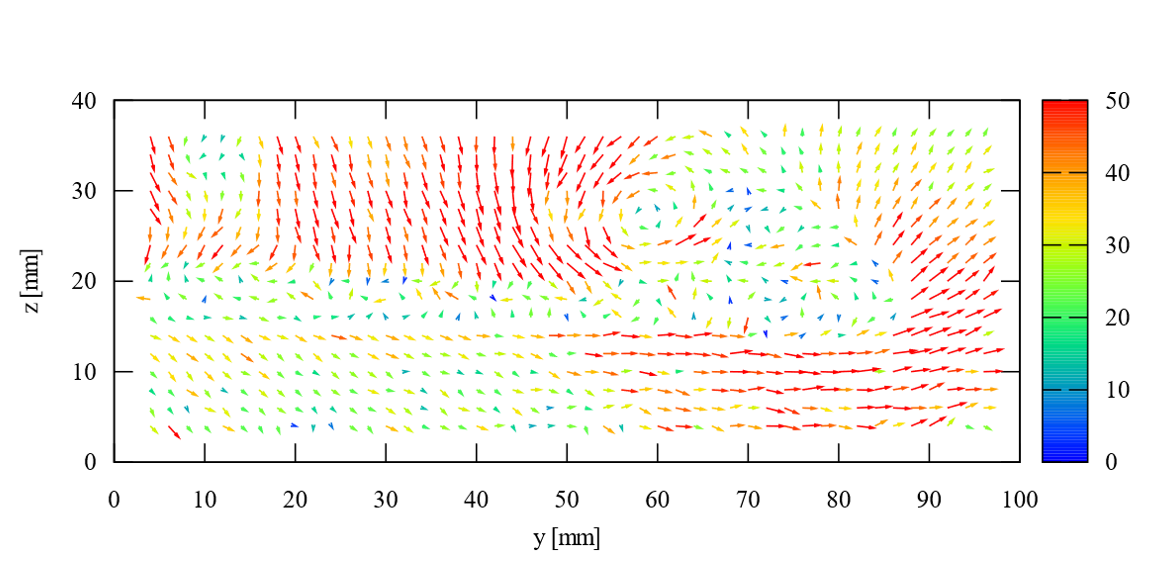
\includegraphics[width=82mm]{../images/right_+5.png}
    \subcaption{Gain $+5$}
    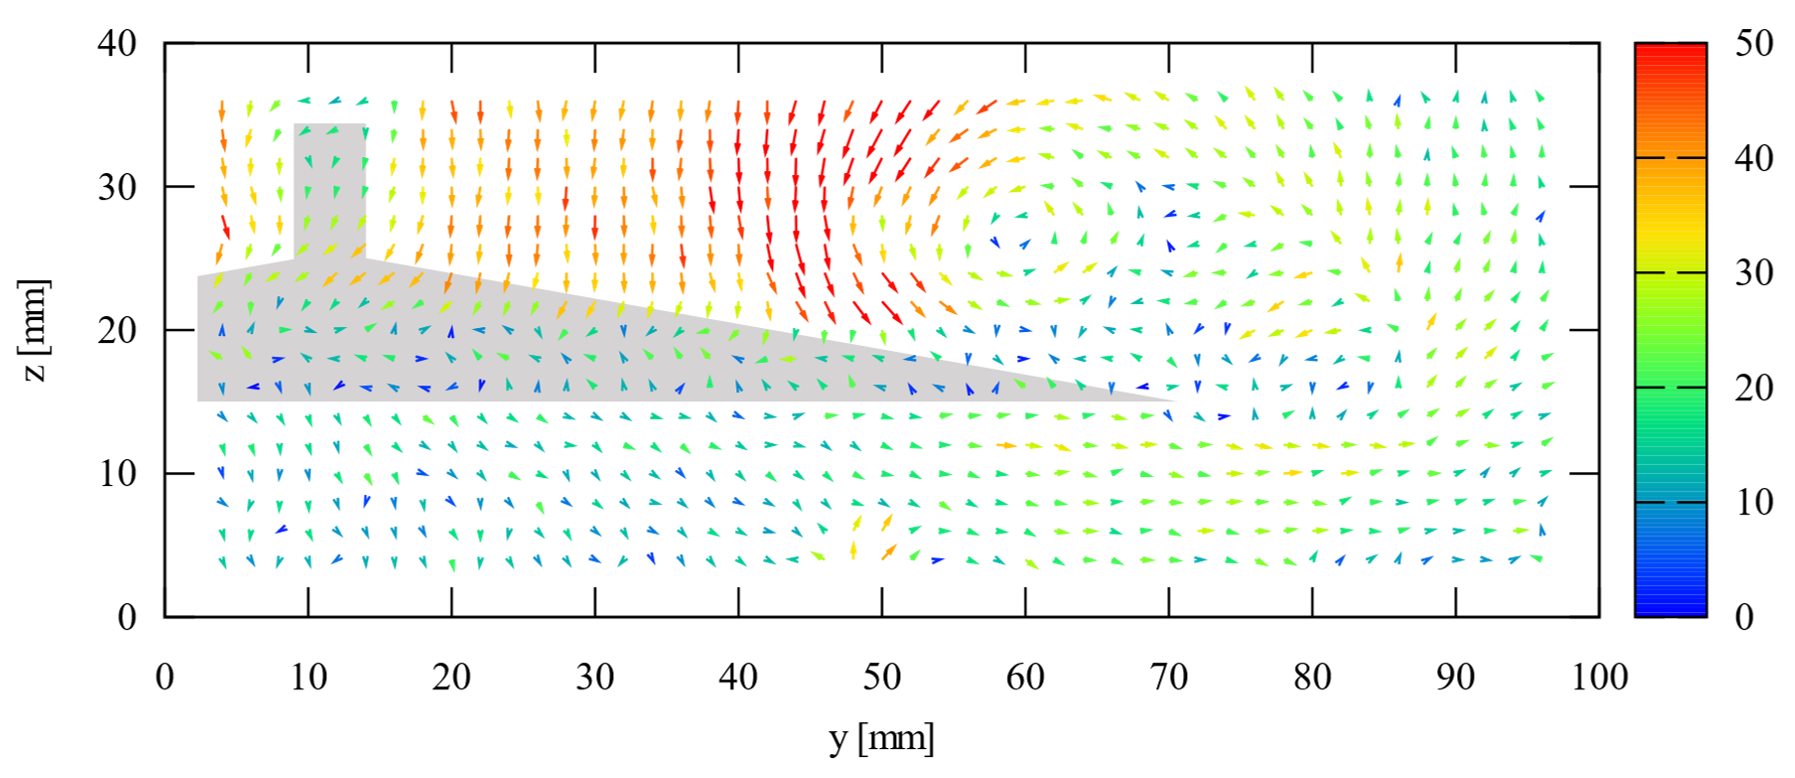
\includegraphics[width=82mm]{../images/right_+10.png}
    \subcaption{Gain $+10$}
  \end{center}
  \caption{PTV time-averaged vectors : $\Delta n = 10$}
\end{figure}

\newpage
\subsection{三角翼後流(1) 中央部}
右翼の解析結果について,渦構造は計測できている.
そこで,流れの対象性を確かめるために中央部の撮影を行った.
それらの解析結果をFig.2に示す.
翼中央の撮影結果より,50mmを中心に
おおよそ左右対称の流れを確認することができる.
しかし,左部の渦については回転を追い切れていない部分があることもわかる.

また,ゲインを変更した結果をみると,ゲインが大きくなるにつれて
速度ベクトルの大きさは小さく評価されていることがわかる.

\begin{figure}[htbp]
  \footnotesize
  \begin{center}
    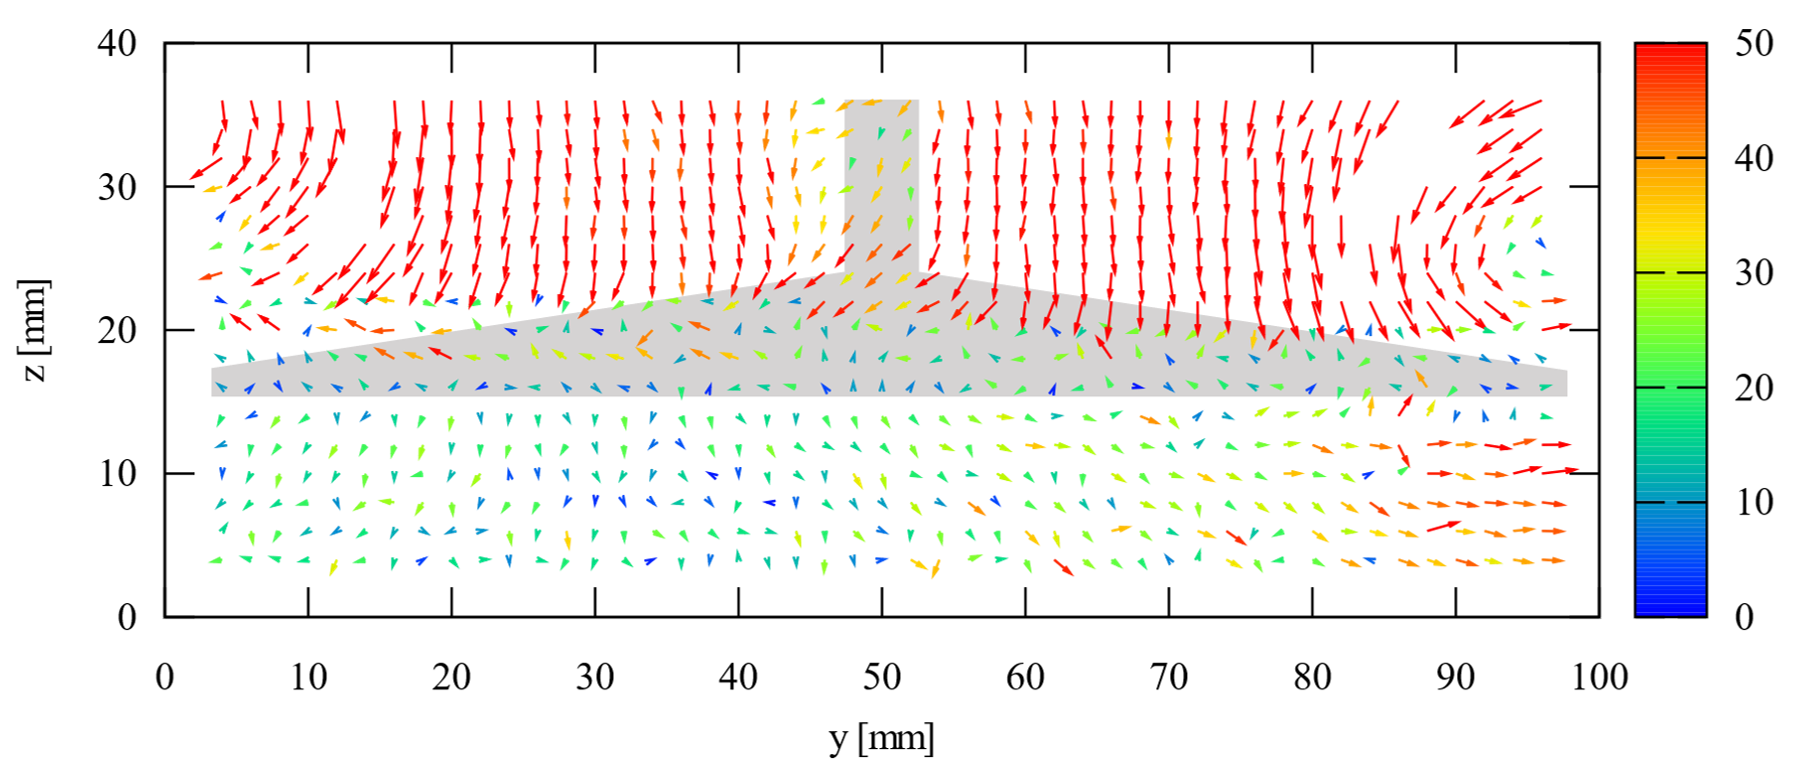
\includegraphics[width=82mm]{../images/center_+0.png}
    \subcaption{Gain $+0$}
    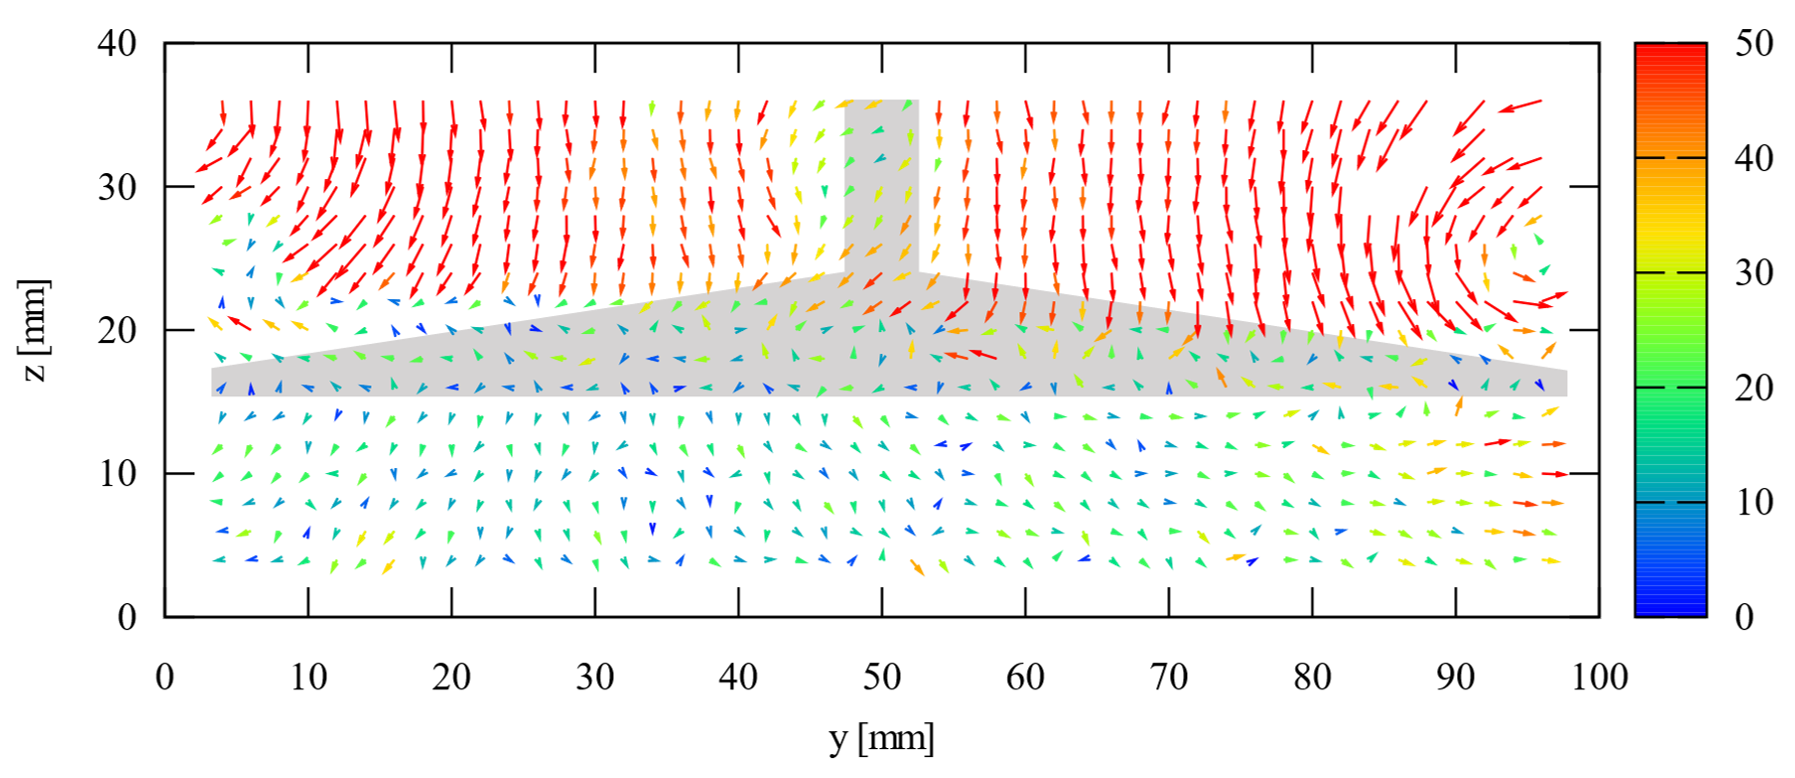
\includegraphics[width=82mm]{../images/center_+5.png}
    \subcaption{Gain $+5$}
    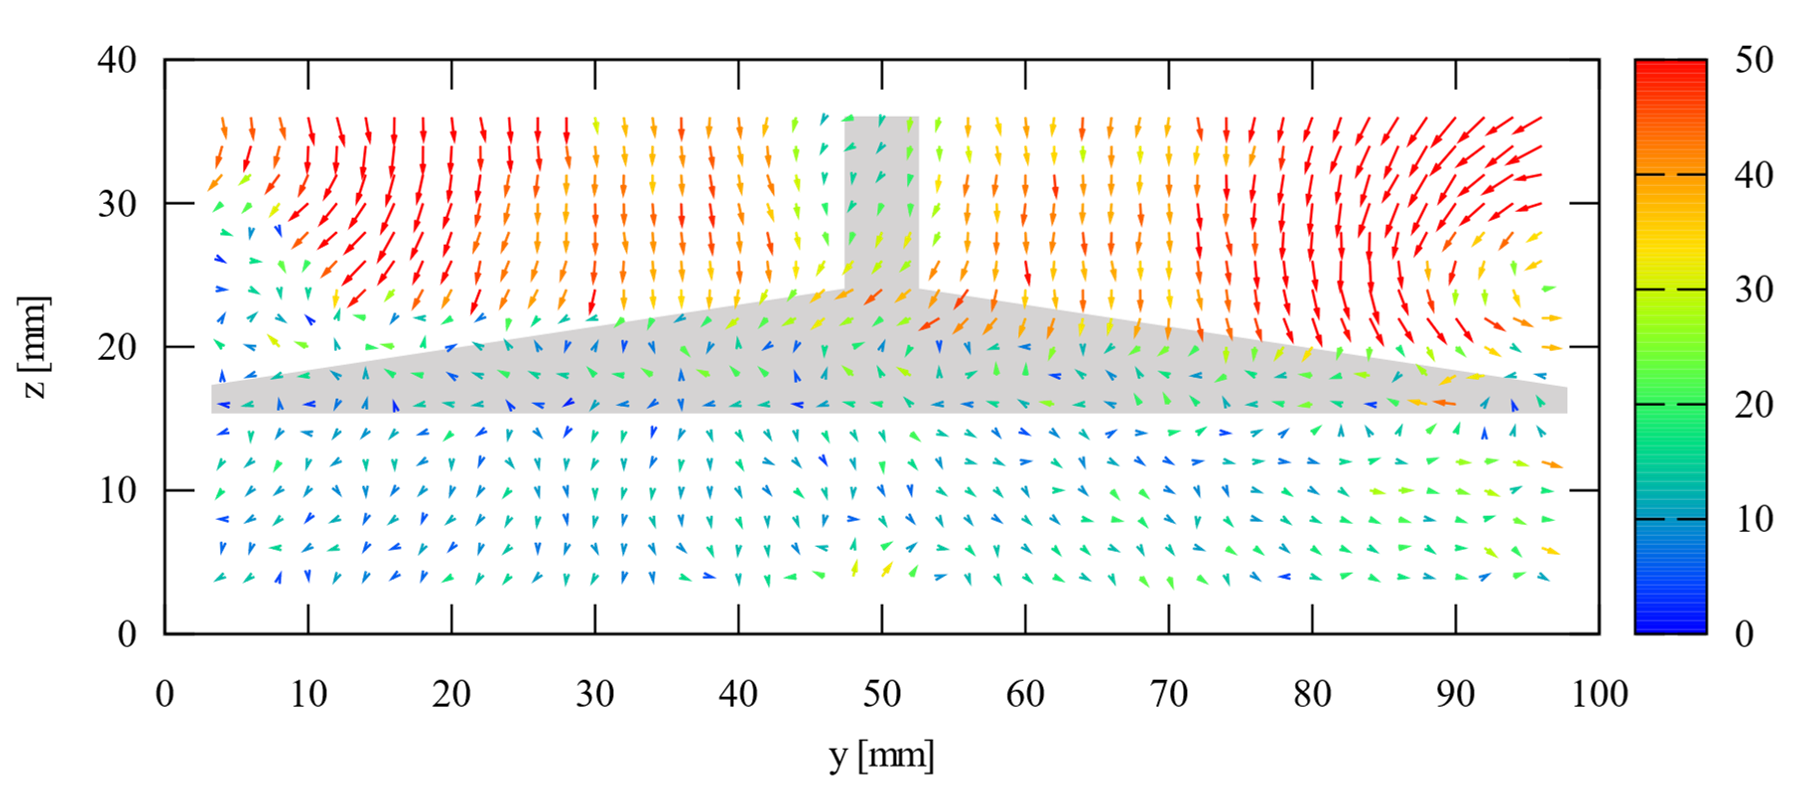
\includegraphics[width=82mm]{../images/center_+10.png}
    \subcaption{Gain $+10$}
  \end{center}
  \caption{PTV time-averaged vectors : $\Delta n = 10$}
\end{figure}



\newpage
\subsection{車両モデル 車軸部}
車両モデルについて,車軸上の流れに示される流れの撮影を行った.
それらの解析結果をFig.3に示す.
以下の結果から,以前の撮影時と同様にホイールハウスとタイヤモデルの空間と
地面板とタイヤモデルの接地部近辺に速度ベクトルが大きくなる箇所があることがわかる.
それに比べ,周囲の速度ベクトルがゼロに近いことから一様流に近いことがわかる.

\begin{figure}[htbp]
  \footnotesize
  \begin{center}
    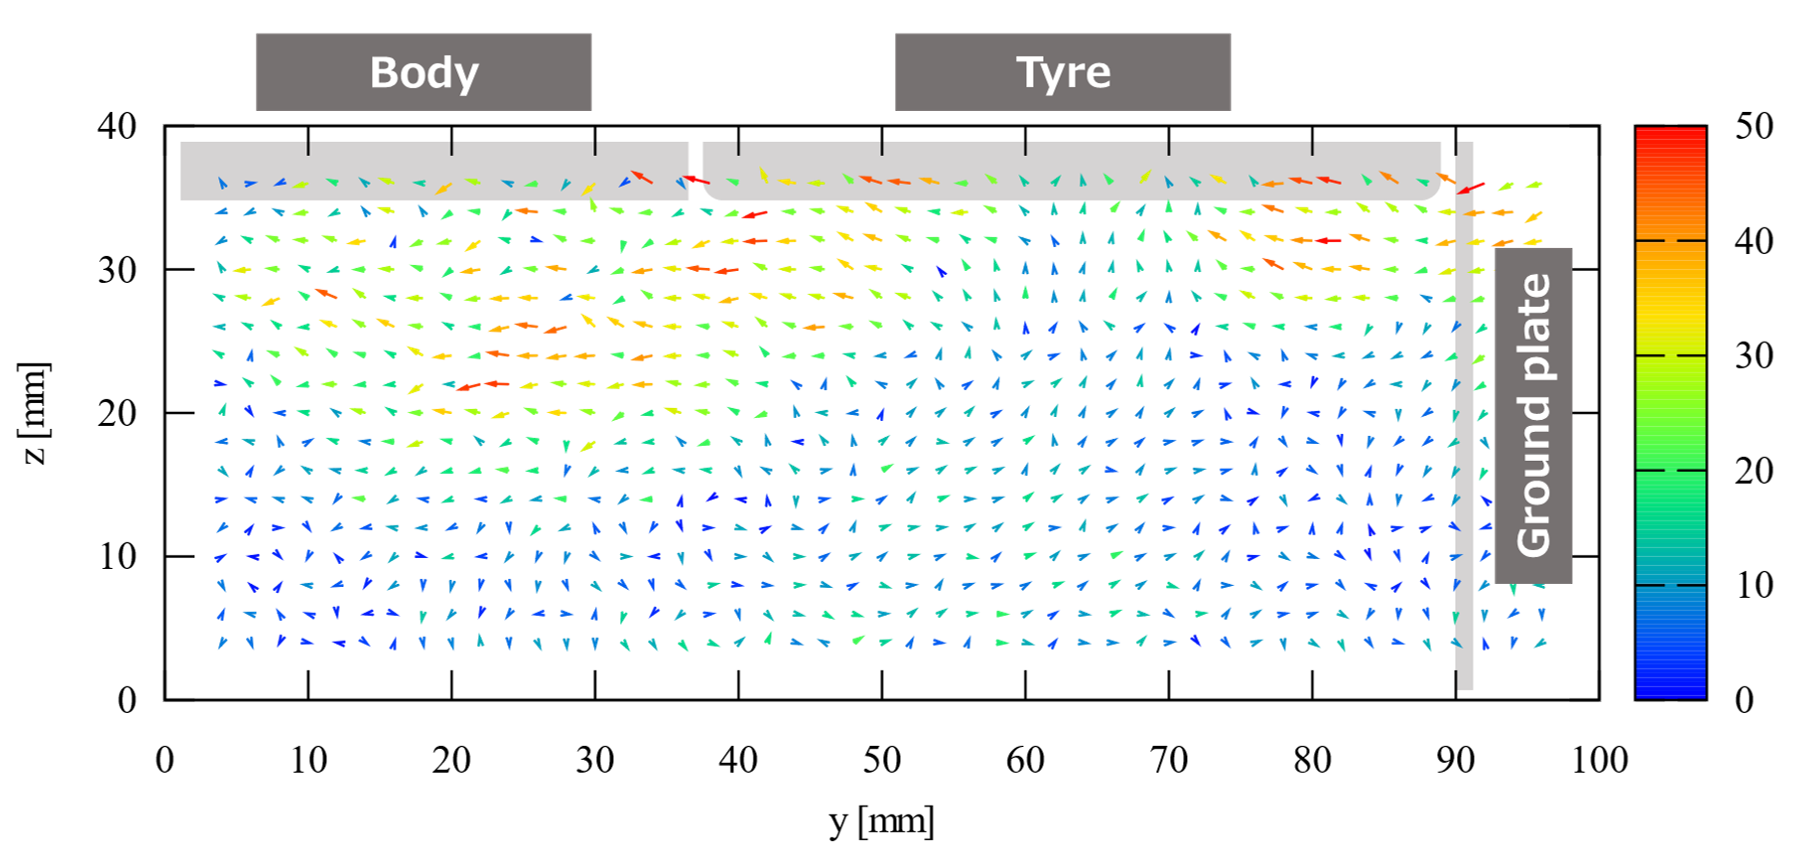
\includegraphics[width=82mm]{../images/tyre_+0.png}
    \subcaption{Gain $+0$}
    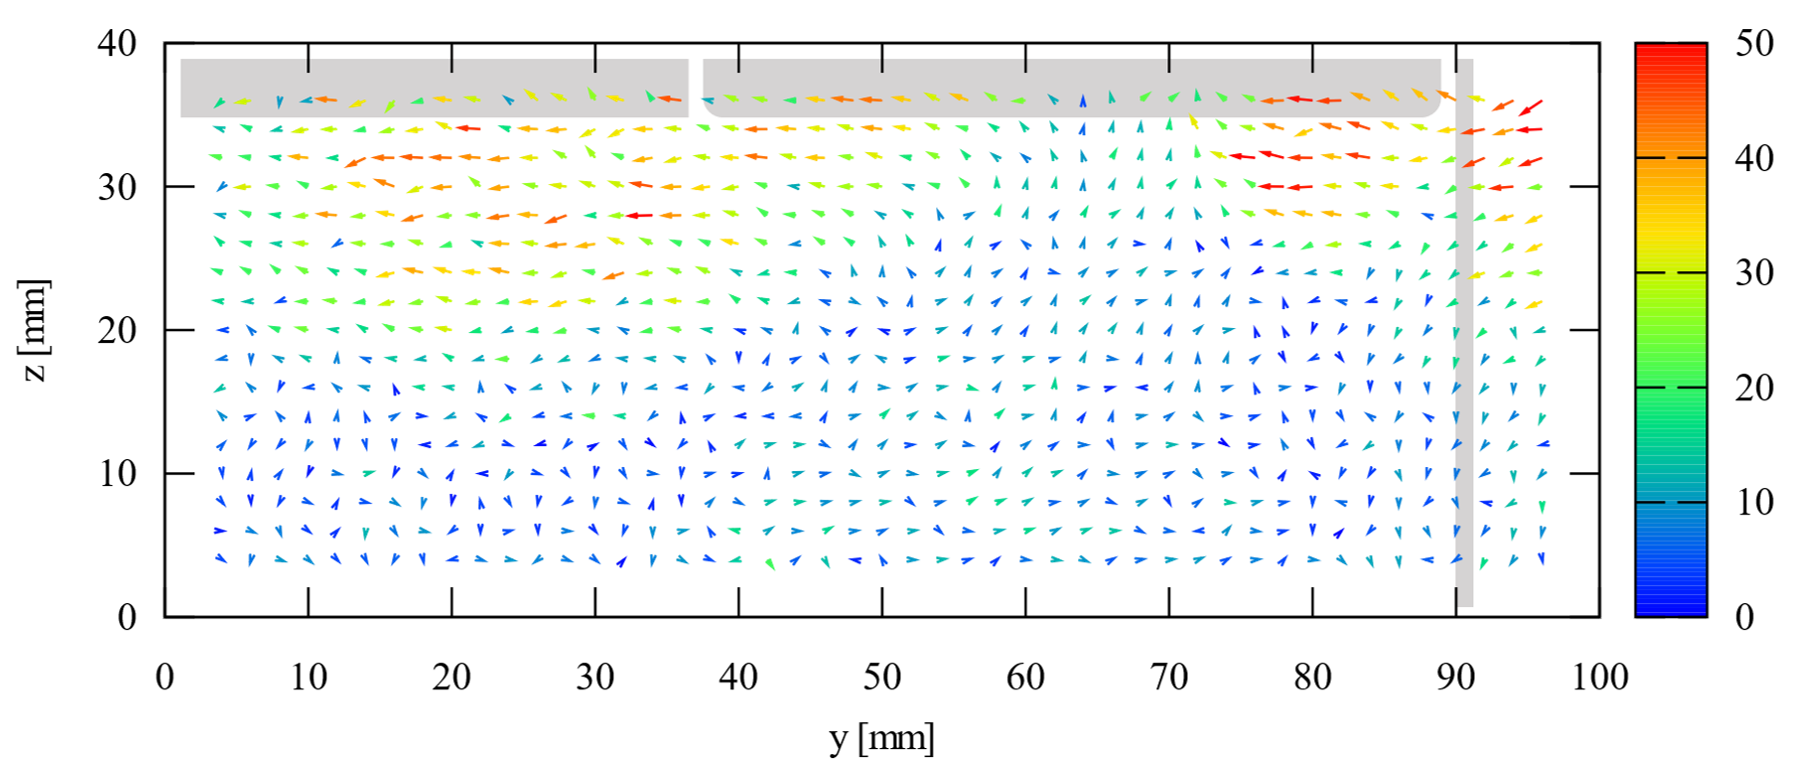
\includegraphics[width=82mm]{../images/tyre_+5.png}
    \subcaption{Gain $+5$}
    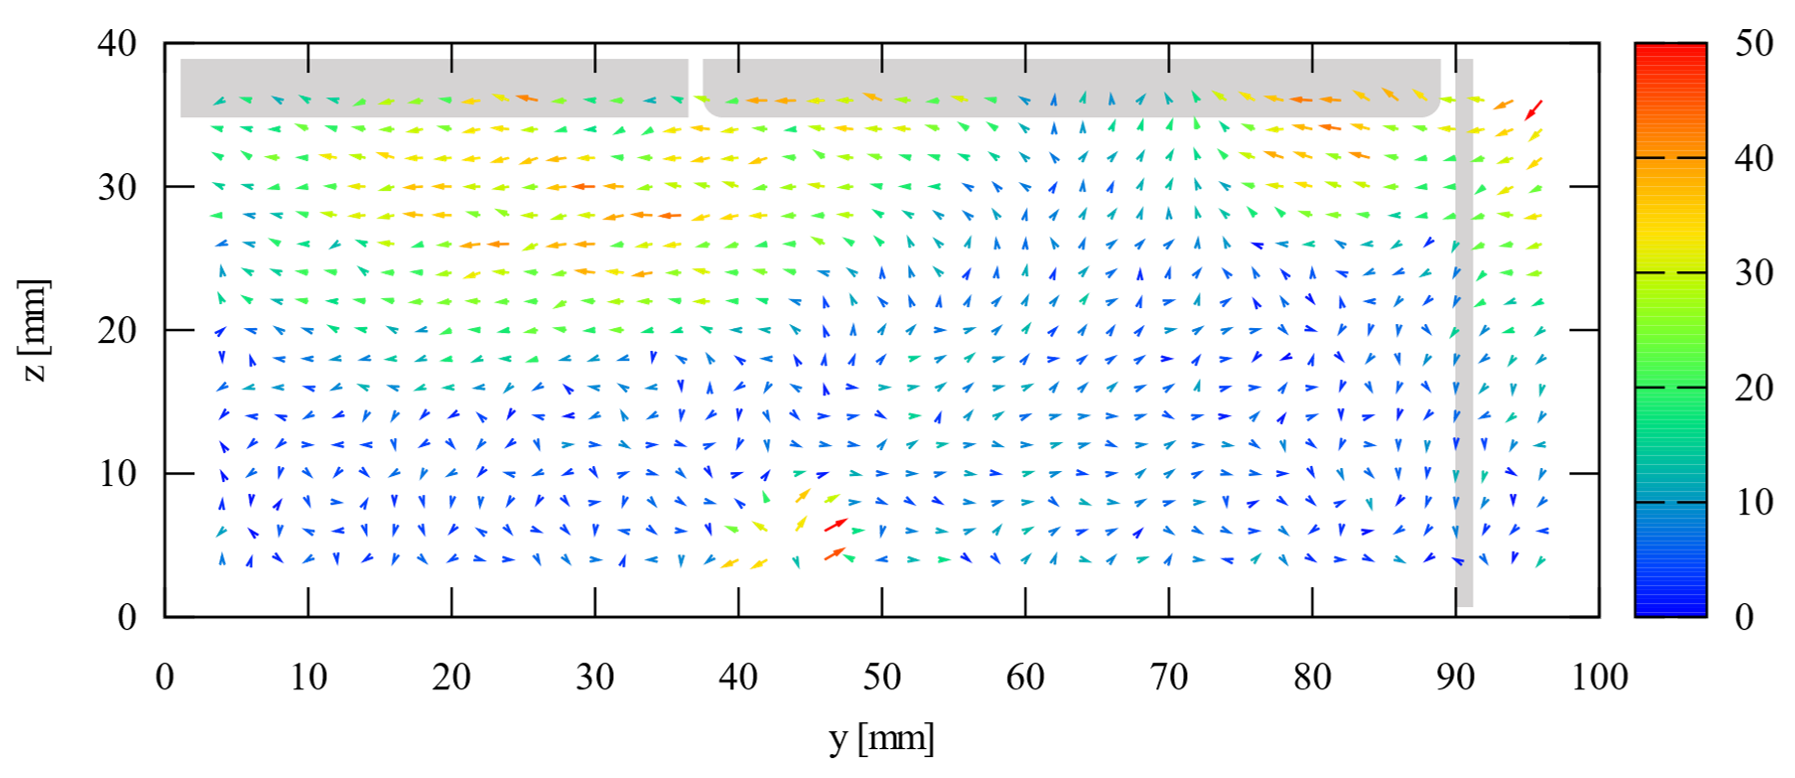
\includegraphics[width=82mm]{../images/tyre_+10.png}
    \subcaption{Gain $+10$}
  \end{center}
  \caption{PTV time-averaged vectors : $\Delta n = 9$}
\end{figure}

\section{可視化情報シンポジウム 資料作成}
報告会にて確認・ご指摘をよろしくお願いいたします.

\section{8月の予定}
\begin{itemize}
  \item 可視化情報シンポジウム (8/8 - 10)
  \item 解析アルゴリズムの改善(対応枚数の判別)
\end{itemize}

\end{document}